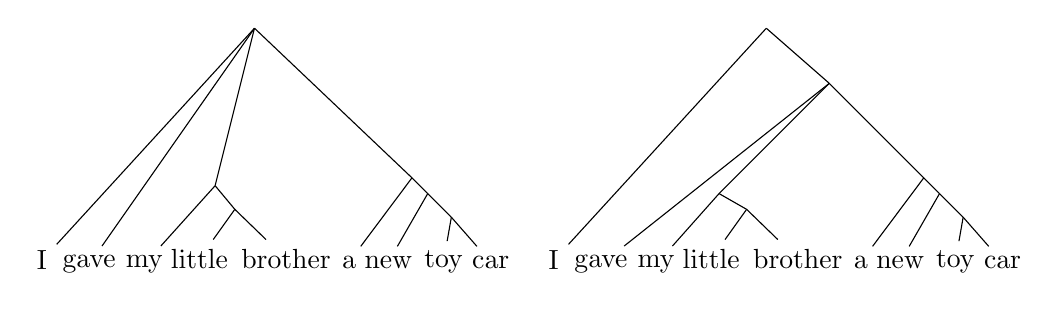
\begin{tikzpicture}

\node (I) at (0,0.05) {I};
\node (gave) at (0.6,0) {gave};
\node (my) at (1.3,0) {my};
\node (little) at (2.0,0.07) {little};
\node (brother) at (3.1,.07) {brother};
\node (a) at (3.9,0.03) {a};
\node (new) at (4.4,0.03) {new};
\node (toy) at (5.1,0.03) {toy};
\node (car) at (5.7,0.03) {car};

\coordinate (toycar) at (5.2,0.6);
\coordinate(newtoycar) at (4.9,0.9);
\coordinate (anewtoycar) at (4.7,1.1);
\coordinate (littlebrother) at (2.45,0.7);
\coordinate (mylittlebrother) at (2.2,1);
\coordinate (all) at (2.7,3);

\foreach \from/\to in {toycar/car, toycar/toy, newtoycar/toycar, newtoycar/new, anewtoycar/newtoycar, anewtoycar/a, littlebrother/brother, littlebrother/little, mylittlebrother/littlebrother, mylittlebrother/my, all/I, all/gave, all/mylittlebrother, all/anewtoycar}
	\draw (\from) -- (\to);

\node (I_) at (6.5,0.05) {I};
\node (gave_) at (7.1,0) {gave};
\node (my_) at (7.8,0) {my};
\node (little_) at (8.5,0.07) {little};
\node (brother_) at (9.6,.07) {brother};
\node (a_) at (10.4,0.03) {a};
\node (new_) at (10.9,0.03) {new};
\node (toy_) at (11.6,0.03) {toy};
\node (car_) at (12.2,0.03) {car};

\coordinate (toycar_) at (11.7,0.6);
\coordinate(newtoycar_) at (11.4,0.9);
\coordinate (anewtoycar_) at (11.2,1.1);
\coordinate (littlebrother_) at (8.95,0.7);
\coordinate (mylittlebrother_) at (8.6,0.9);
\coordinate (gavetobrother_) at (8.1,1.3);
\coordinate (gavetocar_) at (10,2.3);
\coordinate (all_) at (9.2,3);

\foreach \from/\to in {toycar_/car_, toycar_/toy_, newtoycar_/toycar_, newtoycar_/new_, anewtoycar_/newtoycar_, anewtoycar_/a_, littlebrother_/brother_, littlebrother_/little_, mylittlebrother_/littlebrother_, mylittlebrother_/my_, all_/I_, gavetocar_/gave_, gavetocar_/mylittlebrother_, gavetocar_/anewtoycar_, all_/gavetocar_}
	\draw (\from) -- (\to);
\end{tikzpicture}
\caption{Possible compositional structures for the sentence `I gave my little brother a new toy car'}\label{fig:struct2}
